\documentclass[twoside,openany]{SDUthesis}
%\hypersetup{colorlinks=false}
%\makeatletter
%\renewcommand\normalsize{%
%   \@setfontsize\normalsize\@xpt\@xiipt
%   \abovedisplayskip 6\p@ \@plus3\p@ \@minus4\p@
%   \abovedisplayshortskip \z@ \@plus3\p@
%   \belowdisplayshortskip 6\p@ \@plus3\p@ \@minus3\p@
%   \belowdisplayskip \abovedisplayskip
%   \let\@listi\@listI}
%\makeatother

\newcommand{\makeheadrule}{%ҳü
\makebox[0pt][l]{\rule[0.55\baselineskip]{\headwidth}{0.3pt}}
\rule[0.7\baselineskip]{\headwidth}{2.5pt}}
\renewcommand{\headrule}{%
{\if@fancyplain\let\headrulewidth\plainheadrulewidth\fi
\makeheadrule}}
\makeatother

\makeatletter
\newcommand{\figcaption}{\def\@captype{figure}\caption}
\newcommand{\tabcaption}{\def\@captype{table}\caption}
\makeatother

\setlength{\abovecaptionskip}{0pt}
\setlength{\belowcaptionskip}{0pt}

\usepackage{mathrsfs}
\usepackage{pdfpages}
\usepackage{changepage}

%\usepackage{subfigure}
\usepackage{color}
\usepackage{ulem}
\usepackage{graphicx}
\usepackage{subfig}
\usepackage{longtable}
\usepackage{epstopdf}
\usepackage{ccmap}
%\newcommand{\tabincell}[2]{\begin{tabular}{@{}#1@{}}#2\end{tabular}}
%\newcommand{\upcite}[1]{\textsuperscript{\textsuperscript{\cite{#1}}}}

\begin{document}
\raggedbottom

\includepdfmerge{FrontReviewTwo-LCX.pdf,-}

%\makeOSandCPRTpage


\SDUfrontmatter

\SDUcontents
\SDUEcontents

%%%%%%%%%%%%%%%%%%%%%%%%%%%%%%
%% abstract
%%%%%%%%%%%%%%%%%%%%%%%%%%%%%%
\begin{abstract}
\eabstract{Abstract in Chinese}

������ӭ����Ϣ��ը��ʱ���������������������Ƽ��㼰�ƶ��罻ý�����Ϣ������Ѹ�ٷ�չʹ�����ݵ������͹�ģ�������ӣ������ʹ��ģ�����ݶ����ݵĴ����ٶȼ��洢�������涼�и��ߵ����󣬲���Ҫ�ڿɽ���ʱ���ڴ������ģ���ݣ�ͬʱ���ݵĴ洢����ҲҪ�����ڿɳ��ܷ�Χ�ڣ�����ڵ�ǰ���ģ��ģ̬���ݵļ�����Ȼ��һ����ս��Ϊ�˽����ά���ģ���ݵĽ�������ڼ������⣬���ڹ�ϣ�Ľ�������ڼ�������Ӧ�˶�������ϣ������ԭʼ�����ó��ȹ̶��Ķ�ֵ��ϣ������ʾ����ʹ��ԭʼ�����ռ��е������ϵ����������Ϣ�ں����ռ������ɱ��֡�

�������ͳ�Ĺ�ϣ������Ҫ��Ե�ģ̬���ݣ�������ǵ���ģ̬�ڵ����ݼ������⣬��������Ϣ�����Ŀ��ٷ�չ�������ݵı�ը����������ģ̬����Խ��Խ�࣬�����ڶ��ģ̬֮������ݼ������󳡾�Ҳ�������࣬��������ͼ�ȣ���˿�ģ̬��ϣ������Ϊһ����֮��Ч�Ľ��������

Ŀǰ�Ѿ������˶��ֻ��ڻ���ѧϰ�Ŀ�ģ̬��ϣ��������ȡ���˲����ļ���Ч�����������м������������ܵ�������ڣ�1) ���ڶ�ֵ��ɢ�Ż�������ѽ����һЩ��������ɢ���������ɳڣ����������ϣ���ʵֵ��ʾ��֮��Եõ���ʵֵ��ʾ���ж�ֵ���õ����յĹ�ϣ�룬Ȼ�������ɳ��Ż���ʽ������ϴ��������ʹ�����չ�ϣ��ļ���Ч���½���2) ��ǰҲ��һЩ����ֱ�ӽ�����ɢ�Ż�������������ѵ��ʱ��Ϊ���ۣ������Ż�����ʱ�������ӣ�3) �ڼල��Ϣ��ѡ���ϣ��еķ���ѡ��ʹ��\ $n \times n$ �������Ծ�����������Ա��֣�����ᵼ����ѵ����ʱ�临�Ӷȴ�����$O(n)$������$O(n^2)$����������������չ�����ģ���ݼ����Ѷȡ�

�ۺϿ�����������֮�󣬱������һ���мල��ϣ�����������ھ���ֽ�Ŀ���չ��ɢ��ϣ�����Ϊ\ SCRATCH���÷�����Ͼ���ֽ��Լ���ǩǶ������������Ա��ֺͿ���չ�����⣬�������������ת�����������Ż������й�ϣ�����ɢ���ԣ��Ӷ��ɿ��ٵ����ģ��ѵ���������������ȡ�������Ҫ�����ܽ����£�

\begin{itemize}
\vspace{-3mm}
\item ���һ��ȫ�µĻ��ھ���ֽ���мල��ģ̬��ϣ������ͨ������Эͬ����ֽ⣨CMF���ͱ�ǩ����Ƕ�룬\ SCRATCH �ɳ���������еļල������Ϣ���ҵ�һ�������ӿռ䣬ʹ����̬���������֮���������������ܹ�����Ч�ز�׽�����Ӷ������ܵı���ģ̬���ģ̬�ڵ����������ԡ�
\vspace{-3mm}
\item \ SCRATCH ʹ�ñ�ǩ������������Ծ��������ѵ����ʱ�ո��Ӷ�ʼ�������ݼ���ģ����Ϊ���Թ�ϵ���ɷ������չ�����ģ��ģ̬���ݼ��ϡ�
\vspace{-3mm}
\item Ϊ�˱���ʹ���ɳڼ��������ɢ�Ż�������ɵľ޴�������\ SCRATCH �������������ת����ʹ��ѵ��������ʼ�ձ��ֹ�ϣ�����ɢ���ԣ�����ϵ����Ż��IJ��ԣ��Ӷ���С��ѵ�������е���������������ʹ�õ��Ǿ����Ż�����������Ľ����ͨ���󵼵ó����ʽ�⣬��˱�����������ɢ�Ż�����������ѵ��ʱ��Ϊ���۵����⡣
\vspace{-3mm}
\item ͨ����������ģ̬���ݼ��Ͻ��жԱ�ʵ�飬�����������ܡ�ѵ��ʱ���Լ�ʹ�����������ȡͼ��ģ̬�������\ SCRATCH ����ʧ�������뵱ǰ�Ƚ�����ȿ�ģ̬��ϣ�����������ܶԱȣ����Կ������ķ����ڸ���ָ���ϴﵽ��ǰ׿Խ�����ܵ�ͬʱ��ѵ��ʱ���󽵵ͣ��Ӷ����Է������չ�����ģ���ݼ��ϣ����м��ߵ���Ч�Ժ�ʵ���ԡ�
\end{itemize}


\noindent\textbf{�ؼ��ʣ�}��ϣѧϰ����ģ̬����������ֽ⣻��ɢ�Ż�����������ڼ���
%\vspace{0.5em}
%\begin{tabular*}{\textwidth}{ll}
%\hspace{-1em}
%\textbf{�ؼ��ʣ�}& �Ǿֲ������ԣ�ϡ���ԣ�ͼ��ȥ�룻\\
%                &ͼ��ƽ����
%\end{tabular*}
\end{abstract}


%%%%%%%%%%%%%%%%%%%%%%%%%%%%%%
%% english abstract
%%%%%%%%%%%%%%%%%%%%%%%%%%%%%%
\begin{englishabstract}
\eabstract{Abstract in English}

Recent years have witnessed the era of information explosion, in which the rapid development of information technology, i.e., Internet, e-commerce, cloud computing and mobile social media, has led to a sharp increase in the number and size of data. Large-scale multi-modal data put forward higher requirements on data processing and storage capacity, which is not only to process large-scale data in an acceptable time, but also limit the storage capacity of data to an acceptable range. This is still a challenge for the retrieval of large-scale multi-modal data. Hashing emerges in order to solve the problem of approximate nearest neighbor retrieval for high-dimensional large-scale data. It represents the original data  as a fixed-length binary hash code and maintain the original similarity information such as semantic relations in Hamming space.

Most of the traditional hashing methods are mainly designed for single-modal data, which solves the problem of data retrieval in a single modality. With the rapid evolution of information technology and the explosive growth of data, multi-modal data is increasing. Therefore, there are more requirements for cross-modal retrieval, such as using text to retrieve image, and cross-modal hashing retrieval becomes an effective solution.

At present, there are many cross-modal hashing methods based on machine learning, and have achieved great retrieval performance, but there are still some limitations on their performance: As the binary discrete optimization problem is more difficult to solve, some methods relax the discrete conditions by first obtaining the real-valued representation of the hash code, and then binarizing the obtained real-valued representation to obtain the final hash code. However, the relaxation optimization will generate a large quantization error, leading to poor retrieval performance. There are also some methods for direct discrete optimization, but the time required for optimization is greatly increased. In the choice of supervised information, some methods choose to use $n \times n$ similarity matrix for similarity maintaining, which will increase the time complexity of training from linear $O(n)$ to $O(n^2)$, making it harder to extend to large-scale datasets.

After comprehensively taking the above problems into account, this paper proposes a new supervised hashing method, namely, Scalable disCRete mATrix faCtorization Hashing, SCRATCH for short. It combines the collective matrix factorization and semantic embedding to solve the problem of similarity preserving and scalability, and leverages random orthogonal rotation matrix to keep the discrete property of hash codes in training stage, in order to train the model as fast as possible and improve the retrieval precision. The contributions of this work are summarized as follows:

\begin{itemize}
\vspace{-3mm}
\item We propose a novel matrix factorization based supervised cross-modal hashing method. By leveraging the matrix factorization and semantic embedding, SCRATCH can make full use of current supervised semantic information to find a common sub-space where the latent semantic relations among modalities of heterogeneous data can be captured and the intra- and inter-modality similarities are preserved.
\vspace{-3mm}
\item SCRATCH uses label matrix rather than $n \times n$ similarity matrix, such that its time and space complexity are always linear with the number of dataset instances, making it scalable to large-scale datasets.
\vspace{-3mm}
\item In order to avoid the large quantization error caused by using relaxation technique to solve the discrete optimization problem, SCRATCH introduces a random orthogonal rotation matrix to keep the discrete property of hash codes in the training process, and combine with an iterative optimization strategy, thus minimizing the quantization error in the training process. What's more, as it uses matrix optimization techniques, the solution of the matrices can be got by matrix derivation to obtain its closed solution, thus avoiding the large training time of other discrete optimization techniques.
\vspace{-3mm}
\item By comparing experiments on three multi-modal datasets, including retrieval performance, training time, and using a deep network as image feature extractor with loss function of SCRATCH to compare the retrieval performance with current advanced deep cross-modal hashing methods, we can see that SCRATCH achieves state-of-the-art performance on three benchmark multi-modal datasets and the training time is greatly reduced, which means that it is extremely effective and practical and can be easily extended to large-scale datasets.
\end{itemize}


%\vspace{1mm}
%\begin{tabular*}{\textwidth}{ll}
%\hspace{-2.5em}
\noindent\textbf{Keywords:} Hash learning; Cross-modal retrieval; Matrix factorization; Discrete\\
optimization; Approximate nearest neighbor search
%\end{tabular*}

\end{englishabstract}


\SDUmainmatter

%\input{./Chapters/chap0}
\input{./Chapters/chap1}
\input{./Chapters/chap2}
\chapter{\quad\quad ʵ���������}
\label{chap3}
\echapter{Experimental Results and Analyses}

Ϊ����֤��������Ŀ�ģ̬��ϣ��������Ч�ԣ��������������õĻ�׼���ݼ���Wiki\cite{rasiwasia10wiki}��MIRFlickr-25K\cite{huiskes08mir} ��\ NUS-WIDE\cite{chua09nus}�������˽�һ������չʵ�飬����˸���ǰ�Ƚ���dz���ģ̬��ϣ������һ����ȿ�ģ̬��ϣ����������ʵ��Աȡ�ͬʱ��Ϊ�˸��õ�չʾ\ SCRATCH �������Աȷ�������Խ�ԣ�����ʹ��\ MAP ��������������ܣ���������ͬģ̬֮���໥������\ top-N precision ��\ precision-recall ��������һ��˵��\ SCRATCH ����ƶԿ�ģ̬�����������ܵľ޴�������



\section{���ݼ�}
\esection{Datasets}

\textbf{Wiki}�������ݼ��ɴ�\ Wikipedia �ռ���\ 2,866 ��ͼƬ-�ı��Թ��ɣ�����ʮ�����ÿ������ֻ����ʮ���е�һ�࣬���ڵ���ǩ���ݼ�������֮�⣬ÿ��������ͼƬģ̬��\ 128 ά��\ bag-of-visual SIFT ������������ʾ���ı�ģ̬��10ά�����������׷��䣨LDA��������������ʾ����������ݼ��У��������ѡȡ\ $75\%$ ��ͼƬ-�ı�����Ϊѵ�����ͼ�������ʣ���\ $25\%$ ��Ϊ����ѯ���Լ���

\textbf{MIRFlickr-25K}�������ݼ������˴�\ Flickr ���ռ���\ 25,000 ��ͼƬ��ÿ��ͼƬ��24����ͬ���ı���ǩ�е�һ�����������б�ǣ����ڶ��ǩ���ݼ�����ÿ������������һ����ǩ��ǡ�����ѡȡ���������ٰ���20���ı���ǵ�������Ϊʵ�����ݼ���������ѡȡ��\ 20,015 ��������ÿ��������ͼƬģ̬��\ 512 ά��\ GIST ������������ʾ���ı�ģ̬��\ 1,386 ά��\ bag-of-words ������ʾ���ڸ����ݼ��У��������ѡȡ\ 2,000 ��������Ϊ����ѯ���Լ��������\ 18,015 ������������Ϊѵ�����ͼ�������

\textbf{NUS-WIDE}: �����ݼ���\ Flickr ����ȡ��\ 269,648 ��ͼƬ��ÿ���������˹�������ṩ��\ 81 ����ǩ�е�һ��������Ҳ�Ƕ��ǩ���ݼ������ǵ�һЩ��ǩ�õıȽ�ϡ�٣�����ѡȡ��\ 10 ����õı�ǩ�����Ӧ��\ 186,577 ��ͼƬ��Ϊ���յ�ʵ�����ݼ���ÿ��ͼƬ-�ı��Ա����Ϊ\ 10 ���е�����һ�࣬����ÿ��ʵ��������ͼƬģ̬��ʾΪ\ 500 ά��\ bag-of-visual SIFT �����������ı�ģ̬����ʾΪ\ 1,000 ά���������������ڸ����ݼ����������ѡȡ\ 2,000 ��������Ϊ����ѯ���Լ���ʣ���\ 184,577 ��������Ϊѵ�����ͼ�������ֵ��һ����ǣ����ڸ����ݼ�������ģ�ϴ�ͨ�����ڲ��Թ�ϣ�����Ƿ����չ�����ģ���ݼ��ϡ�

\section{�Աȷ��������۱�׼}
\esection{Baselines and Metrics}

���ǽ�\ SCRATCH ����ֵ�ǰ�Ƚ���dz���ģ̬��ϣ��������LSSH\cite{zhouJ14LSSH}��CMFH\cite{ding14cmfh}��SCM-seq\cite{zhang14scm}��CCQ\cite{long16ccq}��SePH-km\cite{lin15seph}��SMFH\cite{Liu16smfh}��FSH\cite{liu17fsh} ��\ DCH\cite{xu17dch}���Լ�һ����ȿ�ģ̬��ϣ��������ȿ�ģ̬��ϣ��DCMH��\cite{jiang2017dcmh}������ʵ��Աȡ���Щ���������Ƿ�ʹ�üල��Ϣ�ɱ�����Ϊ���ࣺLSSH��CMFH��CCQ ��\ FSH ���޼ල��ģ̬��ϣ�������� SCM-seq��SePH-km��SMFH��DCH ��\ DCMH �����мල��ģ̬��ϣ���������жԱȷ�������������ԭ���������ṩ���ڴ˱�ʾ��ֿ��л������֮�⣬SCMFH\cite{ding2016scmfh} ��\ CMFH ���мල��չ�汾��Ȼ��\ SCMFH ԭ����\cite{ding2016scmfh} ����չʾ��ʵ������\ CMFH ��������������ԣ������ķ�����\ CMFH �м����������������\ SCMFH ��Դ������δ��������˱���δ��������Աȷ����С�

��������ض���Щģ�ͽ����˵���ѵ����չʾ����Щģ�����ܴﵽ����ý��������\ NUS-WIDE ���ݼ����ھ޴�SePH-km ��\ FSH ����ʹ����\ $n*n$ �������Ծ��������������������������������ӣ�Ϊ�˽����������������ĸ߶�������������⣬���ǽ�������\ CMFH\cite{ding14cmfh} ��\ SePH-km\cite{lin15seph} ��ʹ�õIJ��ԣ�ͨ����\ NUS-WIDE ѵ���������ѡȡ\ 5,000 ��������ѵ��\ SePH-km ��\ FSH���Ӷ���Сѵ�����ġ�SCRATCH �ĵ��ι��̲��ý�����֤��ѡȡ���ŵij����������ս��Ϊ��$\lambda_1=\lambda_2=0.5$��$\mu=1,000$��$ \alpha=500$��$\gamma=5$������֮�⣬�ܵ�����������Ϊ15 �Ρ�

���з��������ܾ�ʹ��\ Mean Average Precision (MAP)�����ж���������һ������ѯ����\ $\textbf{q}$ ��˵����ƽ�����ȣ�Average Precision��AP����ʾ���£�
\begin{equation}
	AP(q)= \frac{1}{L_q}\sum_{r=1}^nP_q(r)\delta_q(r),
\end{equation}

�����ݿ��У�$L_q$ ������\ $\textbf{q}$ ����ʵ����������$n$ �����ݿ�������������$P_q(r)$ �����˼���ǰ\ $r$ ��������׼ȷ�ʣ������\ $r$ ��������������ʵ���������Ļ�����\ $\delta_q(r)=1$������\ $\delta_q(r)=0$����\ Wiki ����ǩ���ݼ��ϣ���ʵ���ڱ�����Ϊ������ͬ��ǩ����Щ����������\ MIRFlickr-25K ��\ NUS-WIDE ���ݼ��ϣ����Ƕ�����ʵ����Ϊ��Щ���ٹ���һ�������ǩ����������ÿ���������ж����ǩ��ǣ�ֻҪ��һ����ǩ��ͬ����Ϊ���ڣ���

Mean Average Precision (MAP) ����Ϊ��ʽ��
\begin{equation}
	MAP=\frac{1}{|Q|}\sum_{i=1}^{|Q|} AP(q_i),
\end{equation}

����\ $|Q|$ ��������ѯ���Լ�������������


Ϊ�˸�ֱ�۵�չʾ\ SCRATCH �������Աȷ������������������������ǽ�һ�������˸������ݼ��Ϲ�ϣ��λ��Ϊ\ 64 λ��\ 128 λʱ��\ top-N precision ��\ precision-recall ���ߡ���ʵ���У�����̽����������ģ̬��������1) Image-to-Text��ʹ��ͼƬģ̬������Ϊ����ѯ������������Ӧ���ı�ģ̬���ݣ�2) Text-to-Image��ʹ���ı�ģ̬������Ϊ����ѯ������������Ӧ��ͼƬģ̬���ݡ��������еĶ�����׼��˵��MAP ֵԽ������������ڸ߶�Խ�ߣ�������÷���������Խ�á�


\begin{table}[htb]
\small
\center
\begin{center}
\caption{\bf Wiki ���ݼ�����\ MAP �����ܶԱ�}
\label{map_wiki}
%\vspace{-2mm}
\begin{tabular}{cllllll}
  \toprule[1pt]
  Task & Method & 8 bits & 16 bits & 32 bits & 64 bits & 128 bits\\
  \hline
  \multirow{8}{*}{\tabincell{c}{Image\\to\\Text}}
  & {LSSH} & {0.1831} & {0.2162} & {0.2164} & {0.2041} & {0.2084}\\
  & {CMFH} & {0.2006} & {0.2145} & {0.2288} & {0.2360} & {0.2396}\\
  & {SCM-seq} & {0.2125} & {0.2341} & {0.2410} & {0.2437} & {0.2541}\\
  & {CCQ} & {0.1642} & {0.1675} & {0.1683} & {0.1682} & {0.1680}\\
  & {SePH-km} & {0.2620} & {0.2796} &{0.2820} & {0.3076} & {0.3137}\\
  & {SMFH} & {0.1673} & {0.2276} & {0.2470} & {0.2955} & {0.3133}\\
  & {FSH} & {0.1992} & {0.2270} & {0.2433} & {0.2366} & {0.2463}\\
  & {DCH} & {0.3111} & {0.3491} & {0.3589} & {0.3777} & {0.3791}\\
  & {SCRATCH} & {\bf{0.3185}} & {\bf{0.3696}} & {\bf{0.3874}} & {\bf{0.4051}} & {\bf{0.4001}}\\
  \hline
  \multirow{8}{*}{\tabincell{c}{Text\\to\\Image}}
  & {LSSH} & {0.4268} & {0.4990} & {0.5225} & {0.5287} & {0.5330}\\
  & {CMFH} & {0.4434} & {0.4915} & {0.5252} & {0.5276} & {0.5347}\\
  & {SCM-seq} & {0.2013} & {0.2257} & {0.2459} & {0.2480} & {0.2530}\\
  & {CCQ} & {0.2094} & {0.2410} & {0.2518} & {0.2507} & {0.2543}\\
  & {SePH-km} & {0.6065} & {0.6379} & {0.6451} & {0.6662} & {0.6706}\\
  & {SMFH} & {0.3598} & {0.5242} & {0.5961} & {0.6608} & {0.6924}\\
  & {FSH} & {0.4092} & {0.4864} & {0.5197} & {0.4961} & {0.5247}\\
  & {DCH} & {0.6724} & {0.6815} & {0.7097} & {0.7216} & {0.7141}\\
  & {SCRATCH} & {\bf{0.7058}} & {\bf{0.7471}} &{\bf{0.7543}} & {\bf{0.7654}} &{\bf{0.7679}}\\
  \toprule[1pt]
\end{tabular}
\end{center}
\end{table}


\begin{figure*}
%\vspace{-12mm}
\begin{minipage}{0.5\linewidth}
\centering
\centerline{\includegraphics[width=8cm]{figures/Wiki_Precision/Precision_Image_VS_Text_64}}
\end{minipage}
%\vspace{-6mm}
\begin{minipage}{0.5\linewidth}
\centering
\centerline{\includegraphics[width=8cm]{figures/Wiki_Precision/Precision_Text_VS_Image_64}}
\end{minipage}
\caption{\bf Wiki ���ݼ�\ 64 λ��ϣ���\ Top-N precision ����}
\label{curves-wiki-1}\medskip
\end{figure*}

\begin{figure*}
\vspace{-12mm}
\begin{minipage}{0.5\linewidth}
\centering
\centerline{\includegraphics[width=8cm]{figures/Wiki_Precision/Precision_Image_VS_Text_128}}
\end{minipage}
%\vspace{-6mm}
\begin{minipage}{0.5\linewidth}
\centering
\centerline{\includegraphics[width=8cm]{figures/Wiki_Precision/Precision_Text_VS_Image_128}}
\end{minipage}
\caption{\bf Wiki ���ݼ�\ 128 λ��ϣ���\ Top-N precision ����}
\label{curves-wiki-2}\medskip
\end{figure*}



\begin{figure*}
\vspace{-12mm}
\begin{minipage}{0.5\linewidth}
\centering
\centerline{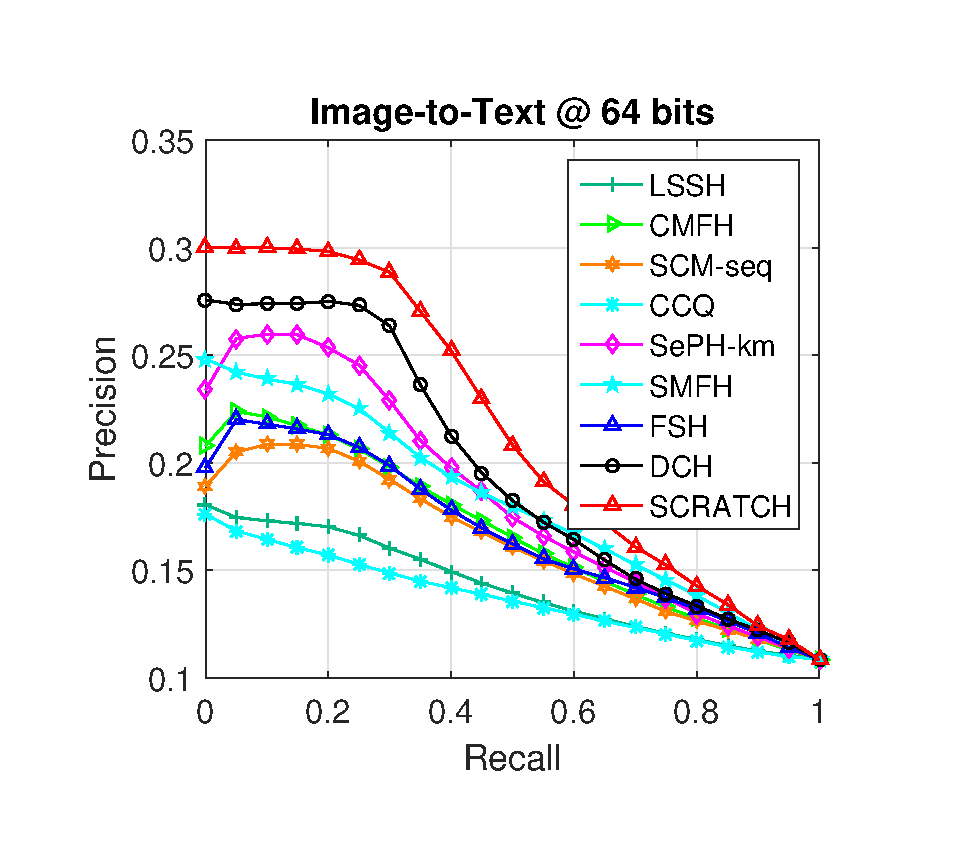
\includegraphics[width=8cm]{figures/WiKi_P_R/P_R_Image_Vs_Text_64}}
\end{minipage}
%\vspace{-6mm}
\begin{minipage}{0.5\linewidth}
\centering
\centerline{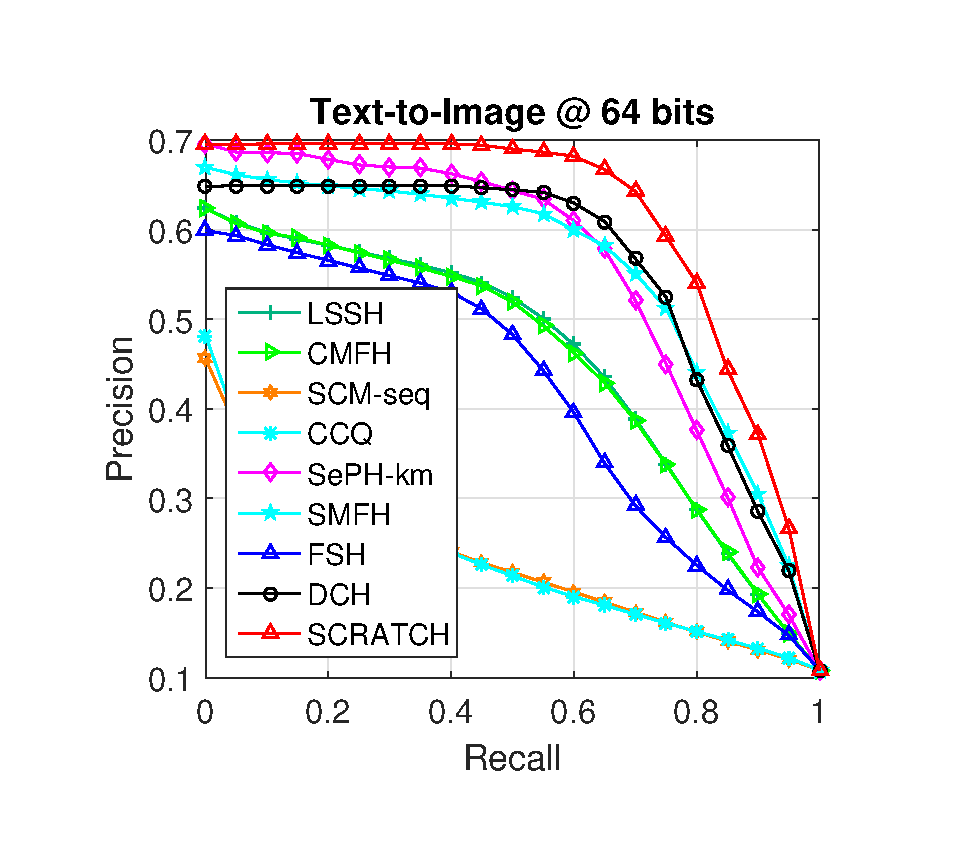
\includegraphics[width=8cm]{figures/WiKi_P_R/P_R_Text_Vs_Image_64}}
\end{minipage}
%\vspace{-4mm}
\caption{\bf Wiki ���ݼ�\ 64 λ��ϣ���\ Precision-Recall ����}
\label{curves-wiki-3}\medskip
\end{figure*}


\begin{figure*}
%\vspace{-12mm}
\begin{minipage}{0.5\linewidth}
\centering
\centerline{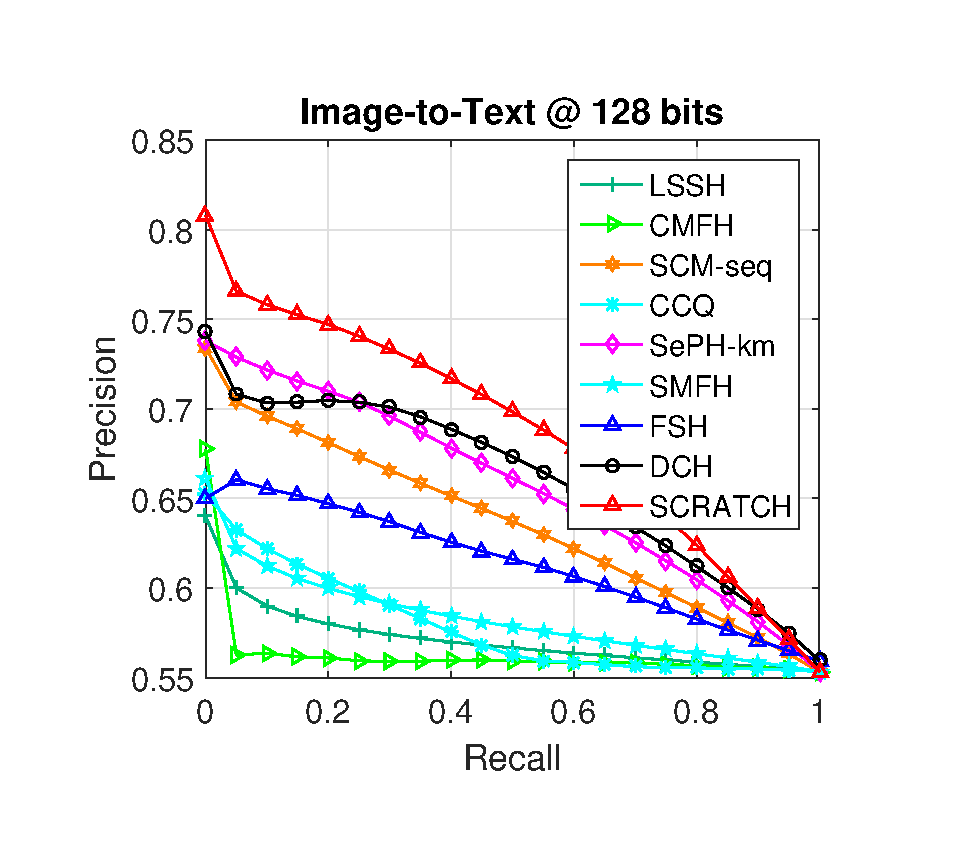
\includegraphics[width=8cm]{figures/Wiki_P_R/P_R_Image_Vs_Text_128}}
\end{minipage}
%\vspace{-6mm}
\begin{minipage}{0.5\linewidth}
\centering
\centerline{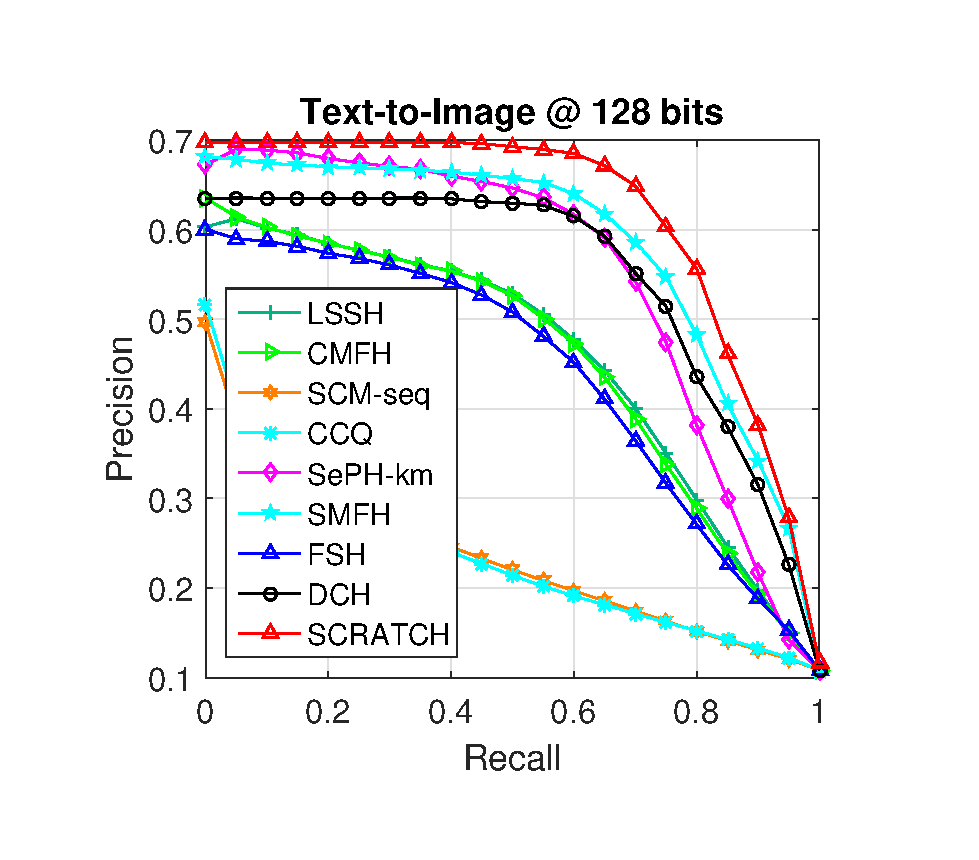
\includegraphics[width=8cm]{figures/WiKi_P_R/P_R_Text_Vs_Image_128}}
\end{minipage}
\caption{\bf Wiki ���ݼ�\ 128 λ��ϣ���\ Precision-Recall ����}
\label{curves-wiki-4}\medskip
\end{figure*}


\section{ʵ���������}
\esection{Results and Analysis}
\label{sec:result}
\subsection{Wiki ���ݼ�ʵ����}
\esubsection{Results on Wiki}
\label{sec:wiki}
SCRATCH �����жԱȷ�����\ Wiki ���ݼ��ϵ�\ MAP ʵ�����ڱ�\ \ref{map_wiki} �н���չʾ��Wiki ���ݼ���\ 64 λ��\ 128 λ��ϣ���ϵ�\ top-N precision ��\ precision-recall ������ͼ \ \ref{curves-wiki-1}��\ref{curves-wiki-4} �л���������Щ��������ǿ��Եó����¼�����ۣ�
%\leftmargini=7mm
%\leftmarginii=6mm
\begin{itemize}
\vspace{-3mm}
\item SCRATCH �ڸ�����ϣ��λ����ִ�����ֿ�ģ̬������������ܶ�Ҫ���������������жԱȷ�����
\vspace{-3mm}
\item ��\ Text-to-Image �����ϣ�SCRATCH ��\ MAP ����ҪԶԶ���������Աȷ��������������������Ҫԭ������������ͼ��ģ̬���ԣ�����ֽ�����״��ı�ģ̬�о�ȷ�ھ������������������Ϣ��
\vspace{-3mm}
\item �����мල��ģ̬��ϣ��������\ SCRATCH��DCH ��\ SePH-km��������ҪԶԶ��Խ�������޼ල��������\ CMFH ��\ FSH������һ��˵��������������Ϣ����Ҫ�ԡ�
\vspace{-3mm}
\item SCRATCH �� $N$ �dz�С��ʱ��Ҫ�������Աȷ������ָ��ã�������\ Image-to-Text �ϣ�����˵��\ SCRATCH ��\ $N$ ��Сʱ�ܹ������������ѯ��������ص����ݿ���������Լ���������˵�Ƿdz���Ҫ�ġ�
\end{itemize}


\begin{table}[htb]
\small
\center
\begin{center}
\caption{\bf MIRFlickr-25K ���ݼ�����\ MAP �����ܶԱ�}
\label{mAP_flickr}
%\vspace{-2mm}
\begin{tabular}{cllllll}
  \toprule[1pt]
  Task & Method & 8 bits & 16 bits & 32 bits & 64 bits & 128 bits\\
  \hline
  \multirow{8}{*}{\tabincell{c}{Image\\to\\Text}}
  & {LSSH} & {0.5698} & {0.5812} & {0.5811} & {0.5805} & {0.5800}\\
  & {CMFH} & {0.5599} & {0.5687} & {0.5680} & {0.5685} & {0.5687}\\
  & {SCM-seq} & {0.6235} & {0.6373} & {0.6478} & {0.6537} & {0.6611}\\
  & {CCQ} & {0.5712} & {0.5885} & {0.5908} & {0.5924} & {0.5928}\\
  & {SePH-km} & {0.6641} & {0.6685} &{0.6818} & {0.6830} & {0.6873}\\
  & {SMFH} & {0.5587} & {0.5688} & {0.5917} & {0.5953} & {0.5961}\\
  & {FSH} & {0.5911} & {0.6016} & {0.6149} & {0.6194} & {0.6242}\\
  & {DCH} & {0.6659} & {0.6738} & {0.6859} & {0.6897} & {0.7030}\\
  & {SCRATCH} & {\bf{0.7092}} & {\bf{0.7131}} &{\bf{0.7222}} & {\bf{0.7265}} &{\bf{0.7346}}\\
  \hline
  \multirow{8}{*}{\tabincell{c}{Text\\to\\Image}} %$T\rightarrow I$
  & {LSSH} & {0.5914} & {0.5917} & {0.5929} & {0.5926} & {0.5918}\\
  & {CMFH} & {0.5615} & {0.5615} & {0.5606} & {0.5606} & {0.5608}\\
  & {SCM-seq} & {0.6103} & {0.6206} & {0.6298} & {0.6372} & {0.6427}\\
  & {CCQ} & {0.5902} & {0.5970} & {0.5992} & {0.6001} & {0.6001}\\
  & {SePH-km} & {0.7033} & {0.7076} & {0.7212} & {0.7293} & {0.7348}\\
  & {SMFH} & {0.5568} & {0.5586} & {0.5727} & {0.5841} & {0.5828}\\
  & {FSH} & {0.5869} & {0.5979} & {0.6114} & {0.6186} & {0.6251}\\
  & {DCH} & {0.7256} & {0.7511} & {0.7585} & {0.7681} & {0.7909}\\
  %& {DCH} & {0.7344} & {0.7425} & {0.7599} & {0.7633} & {0.7927}\\
  & {SCRATCH} & {\bf{0.7591}} & {\bf{0.7762}} &{\bf{0.7822}} & {\bf{0.7978}} & {\bf{0.8063}}\\
  \toprule[1pt]
\end{tabular}
\end{center}
\end{table}

\subsection{MIRFlickr-25K ���ݼ�ʵ����}
\esubsection{Results on MIRFlickr-25K}
\label{sec:mirflickr}

MIRFlickr-25K ���ݼ���\ Image-to-Text ��\ Text-to-Image ������ģ̬���������\ MAP ʵ�����ڱ�\ \ref{mAP_flickr} �н������ܽᣬ�����ݼ���\ 64 λ��\ 128 λ��ϣ���ϵ�\ top-N precision ��\ precision-recall ������ͼ\ \ref{curves-flickr-1}��\ref{curves-flickr-4} �л�����ͨ������������\ MIRFlickr-25K ���ݼ��ϵ�ʵ���������ǿ��Թ۲쵽���漸�㣺
\begin{itemize}
\vspace{-3mm}
\item ����\ Wiki ���ݼ��ϵĽ����ͬ��SCRATCH �ڸ�����ϣ��λ����ִ�����ֿ�ģ̬������������ܶ�Ҫ���������������жԱȷ�����
\vspace{-3mm}
\item SCRATCH �ڹ�ϣ��λ���ܵͣ���\ 8 ��\ 16 λ����ʱ����Ȼȡ����Զ���������Աȷ����ļ������ܣ�����ζ�Ŷ��ڸ�ά������˵��SCRATCH ���Խ��併ά�����͵�ά�Ƚ��м�����ͬʱ��֤������������Ӷ�������������Ⱥ��ٶȡ�
\vspace{-3mm}
\item ���Ź�ϣ��λ�����ӣ�SCRATCH �ļ������ܳ���������˵�������Ĺ�ϣ���ܹ���������Ϣ�������ϣ���У��Ӷ�ʵ�ּ������ܵĿ���������
\vspace{-3mm}
\item һ����˵�������������\ Text-to-Image �����ϵļ�������ҪԶԶ����\ Image-to-Text ���񣬿��ܵ�ԭ�������ı���ͼ��������������������ı�-ͼ������������⣬�Ӷ�����ʹ���ı�������ͼ��������ס�
\vspace{-3mm}
\item ��\ Wiki ���ݼ��ϵ�ʵ������ȣ���\ MIRFlickr-25K ���ݼ������еķ�����ȡ���˸��õؼ������ܣ�������������������ݼ���ʹ�õ�������ʾ������ͬ��ͬʱ��ͬ�����ݼ������ݷֲ�Ҳ������ͬ��������ͬ�����ڲ�ͬ���ݼ��ϵļ��������������졣
\end{itemize}



\begin{figure*}
%\vspace{-12mm}
\begin{minipage}{0.5\linewidth}
\centering
\centerline{\includegraphics[width=8cm]{figures/FLICKR_Precision/Precision_Image_VS_Text_64}}
\end{minipage}
%\vspace{-6mm}
\begin{minipage}{0.5\linewidth}
\centering
\centerline{\includegraphics[width=8cm]{figures/FLICKR_Precision/Precision_Text_VS_Image_64}}
\end{minipage}
\caption{\bf MIRFlickr-25K ���ݼ�\ 64 λ��ϣ���\ Top-N precision ����}
\label{curves-flickr-1}\medskip
\end{figure*}


\begin{figure*}
\vspace{-6mm}
\begin{minipage}{0.5\linewidth}
\centering
\centerline{\includegraphics[width=8cm]{figures/FLICKR_Precision/Precision_Image_VS_Text_128}}
\end{minipage}
%\vspace{-6mm}
\begin{minipage}{0.5\linewidth}
\centering
\centerline{\includegraphics[width=8cm]{figures/FLICKR_Precision/Precision_Text_VS_Image_128}}
\end{minipage}
\caption{\bf MIRFlickr-25K ���ݼ�\ 128 λ��ϣ���\ Top-N precision ����}
\label{curves-flickr-2}\medskip
\end{figure*}


\begin{figure*}
%\vspace{-12mm}
\begin{minipage}{0.5\linewidth}
\centering
\centerline{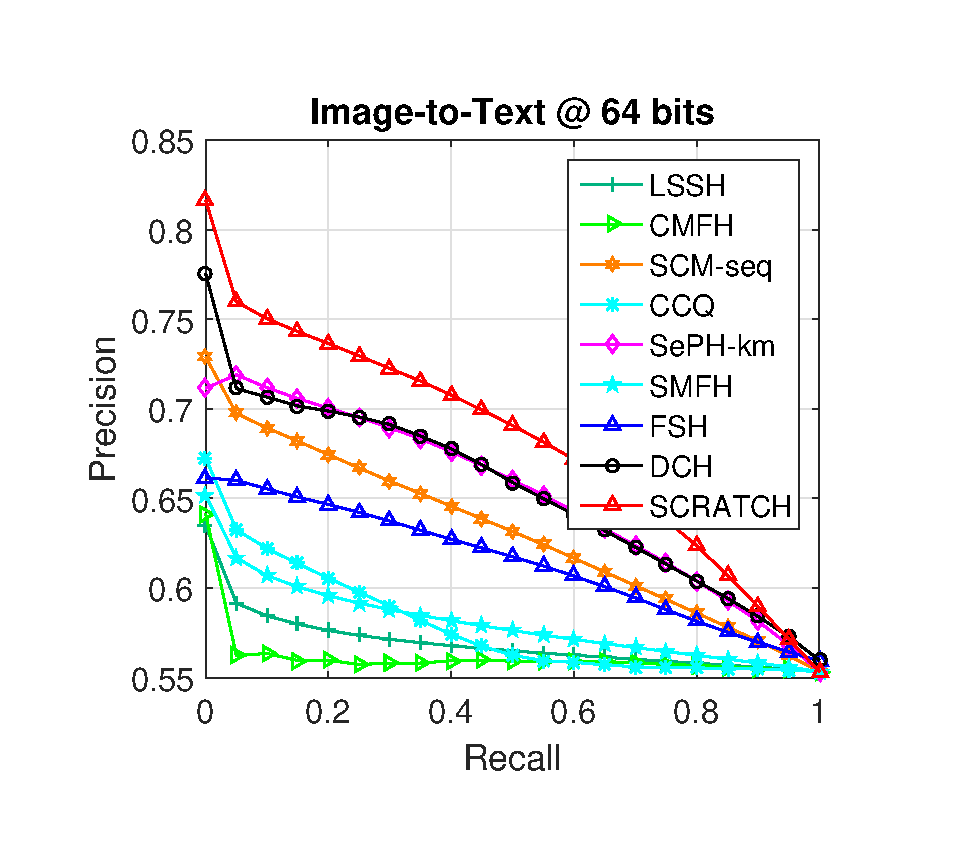
\includegraphics[width=8cm]{figures/FLICKR_P_R/P_R_Image_Vs_Text_64}}
\end{minipage}
%\vspace{-6mm}
\begin{minipage}{0.5\linewidth}
\centering
\centerline{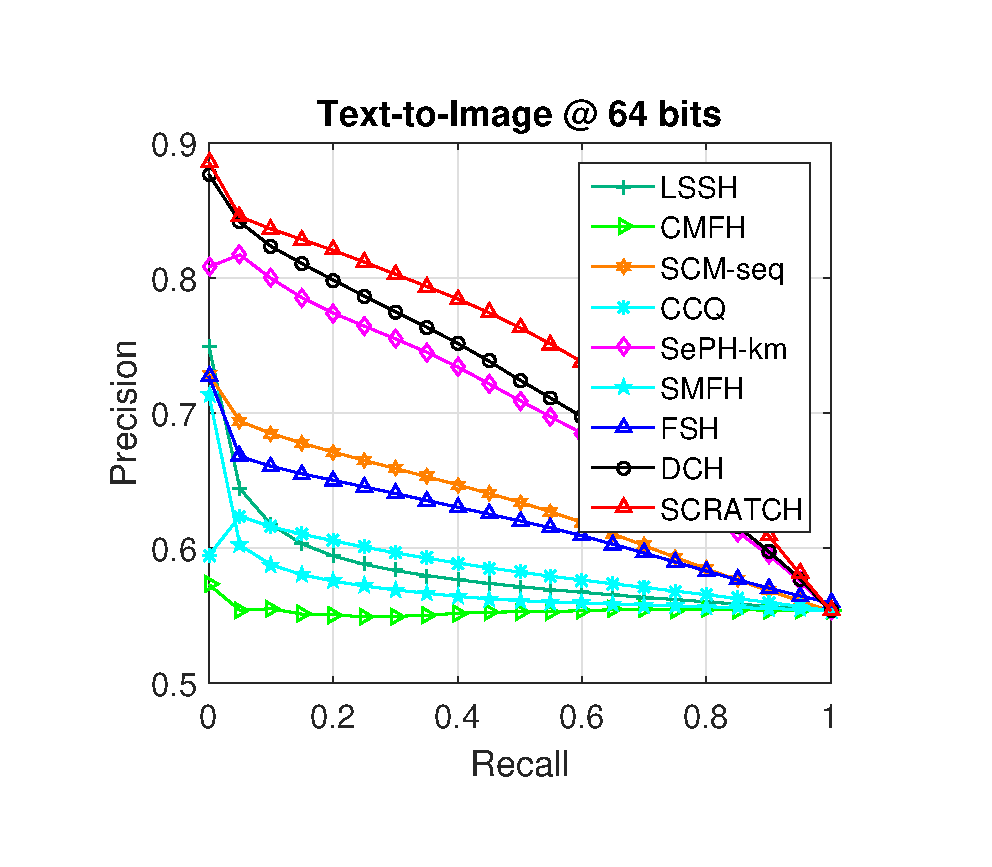
\includegraphics[width=8cm]{figures/FLICKR_P_R/P_R_Text_Vs_Image_64}}
\end{minipage}
%\vspace{-4mm}
\caption{\bf MIRFlickr-25K ���ݼ�\ 64 λ��ϣ���\ Precision-Recall ����}
\label{curves-flickr-3}\medskip
\end{figure*}


\begin{figure*}
\vspace{-12mm}
\begin{minipage}{0.5\linewidth}
\centering
\centerline{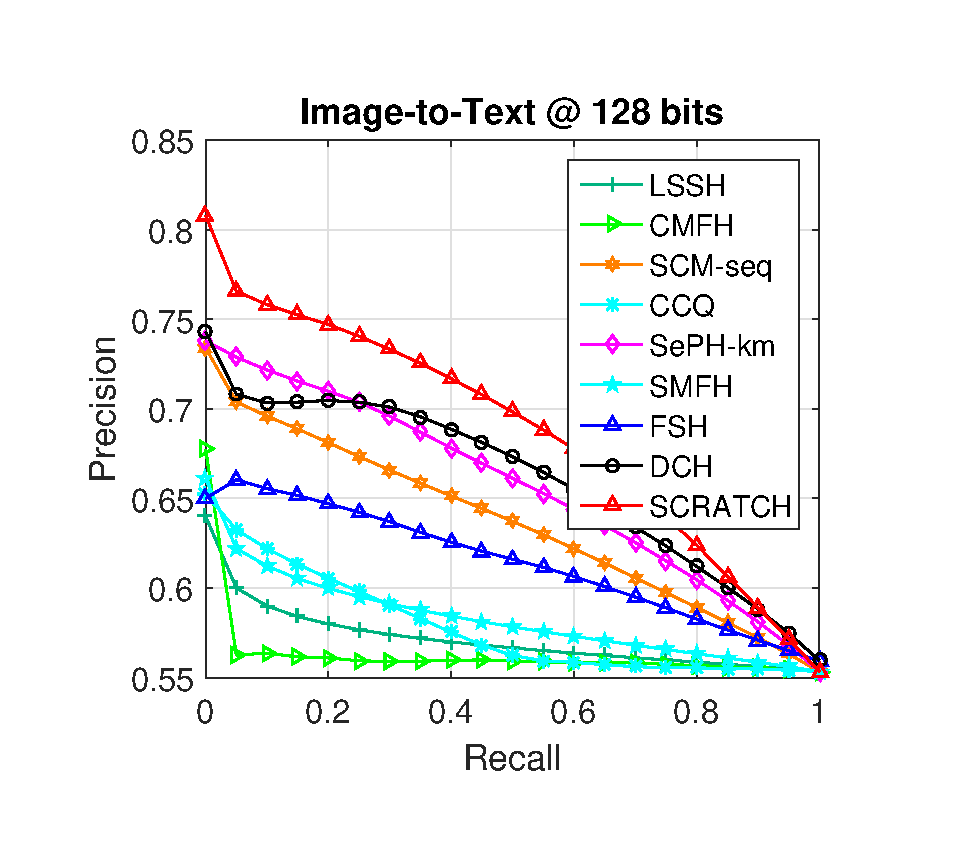
\includegraphics[width=8cm]{figures/Wiki_P_R/P_R_Image_Vs_Text_128}}
\end{minipage}
%\vspace{-6mm}
\begin{minipage}{0.5\linewidth}
\centering
\centerline{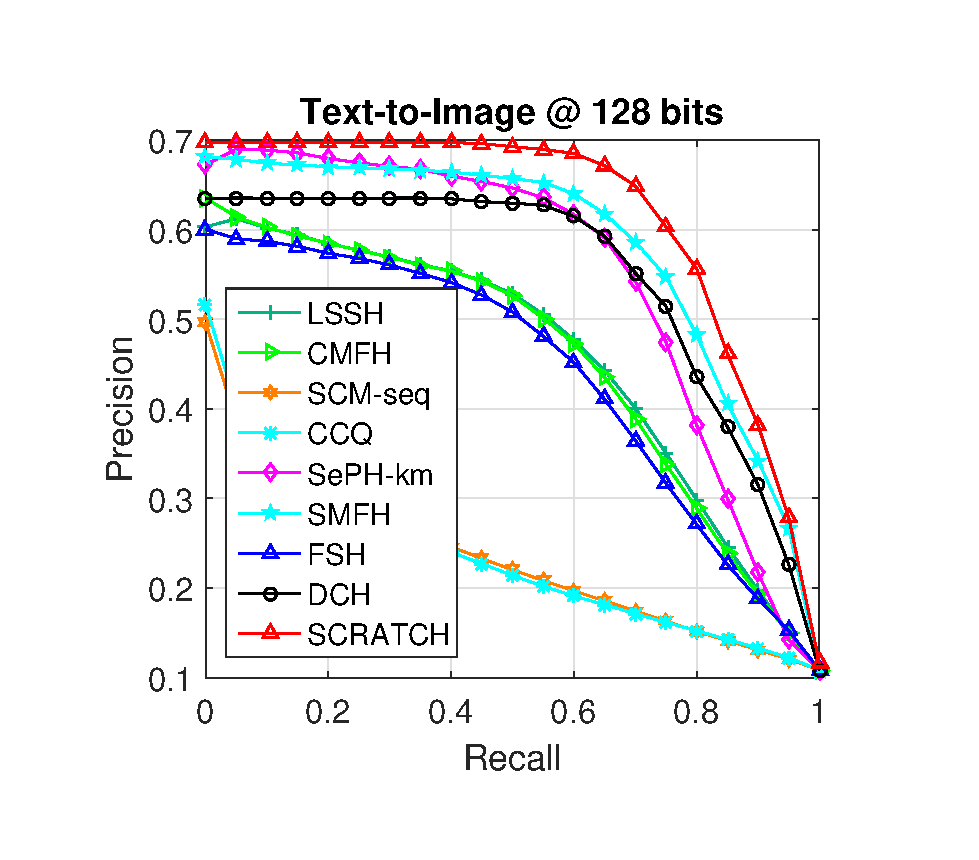
\includegraphics[width=8cm]{figures/WiKi_P_R/P_R_Text_Vs_Image_128}}
\end{minipage}
\caption{\bf MIRFlickr-25K ���ݼ�\ 128 λ��ϣ���\ Precision-Recall ����}
\label{curves-flickr-4}\medskip
\end{figure*}


\begin{figure*}
\vspace{-12mm}
\begin{minipage}{0.5\linewidth}
\centering
\centerline{\includegraphics[width=8cm]{figures/NUS_WIDE_Precision/Precision_Image_VS_Text_64}}
\end{minipage}
%\vspace{-6mm}
\begin{minipage}{0.5\linewidth}
\centering
\centerline{\includegraphics[width=8cm]{figures/NUS_WIDE_Precision/Precision_Text_VS_Image_64}}
\end{minipage}
\caption{\bf NUS-WIDE ���ݼ�\ 64 λ��ϣ���\ Top-N precision ����}
\label{curves-nus-1}\medskip
\end{figure*}

\begin{figure*}
%\vspace{-12mm}
\begin{minipage}{0.5\linewidth}
\centering
\centerline{\includegraphics[width=8cm]{figures/NUS_WIDE_Precision/Precision_Image_VS_Text_128}}
\end{minipage}
%\vspace{-6mm}
\begin{minipage}{0.5\linewidth}
\centering
\centerline{\includegraphics[width=8cm]{figures/NUS_WIDE_Precision/Precision_Text_VS_Image_128}}
\end{minipage}
\caption{\bf NUS-WIDE ���ݼ�\ 128 λ��ϣ���\ Top-N precision ����}
\label{curves-nus-2}\medskip
\end{figure*}



\begin{figure*}
\vspace{-12mm}
\begin{minipage}{0.5\linewidth}
\centering
\centerline{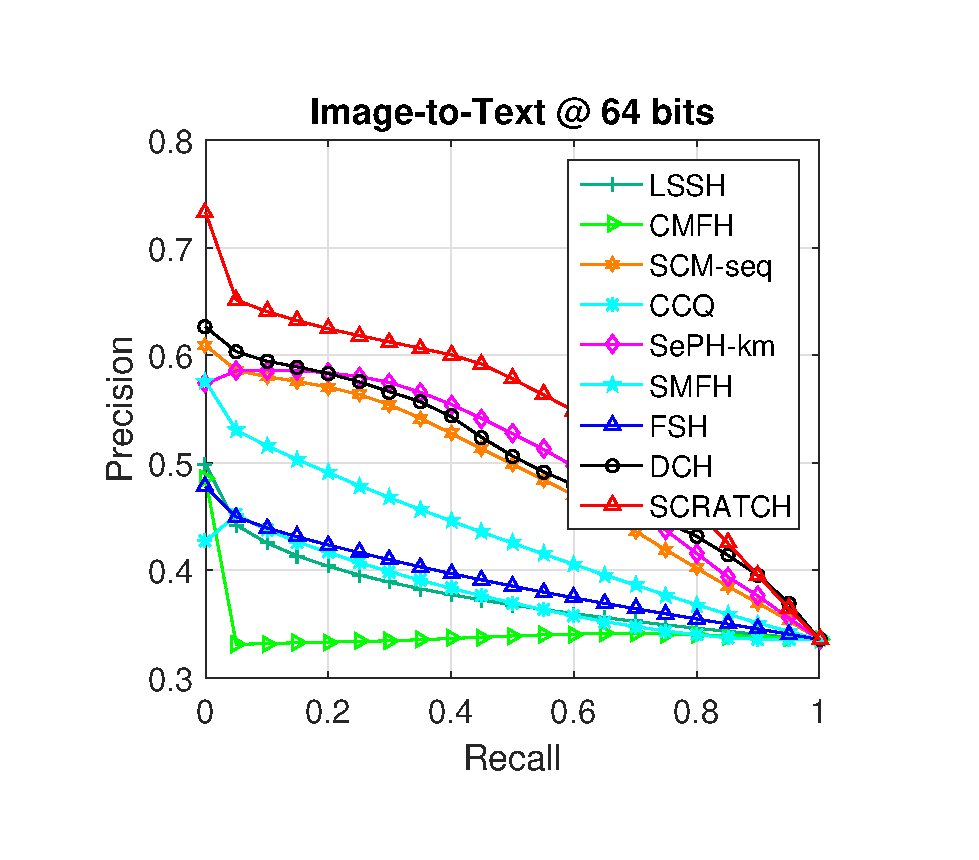
\includegraphics[width=8cm]{figures/NUS_WIDE_P_R/P_R_Image_Vs_Text_64}}
\end{minipage}
%\vspace{-6mm}
\begin{minipage}{0.5\linewidth}
\centering
\centerline{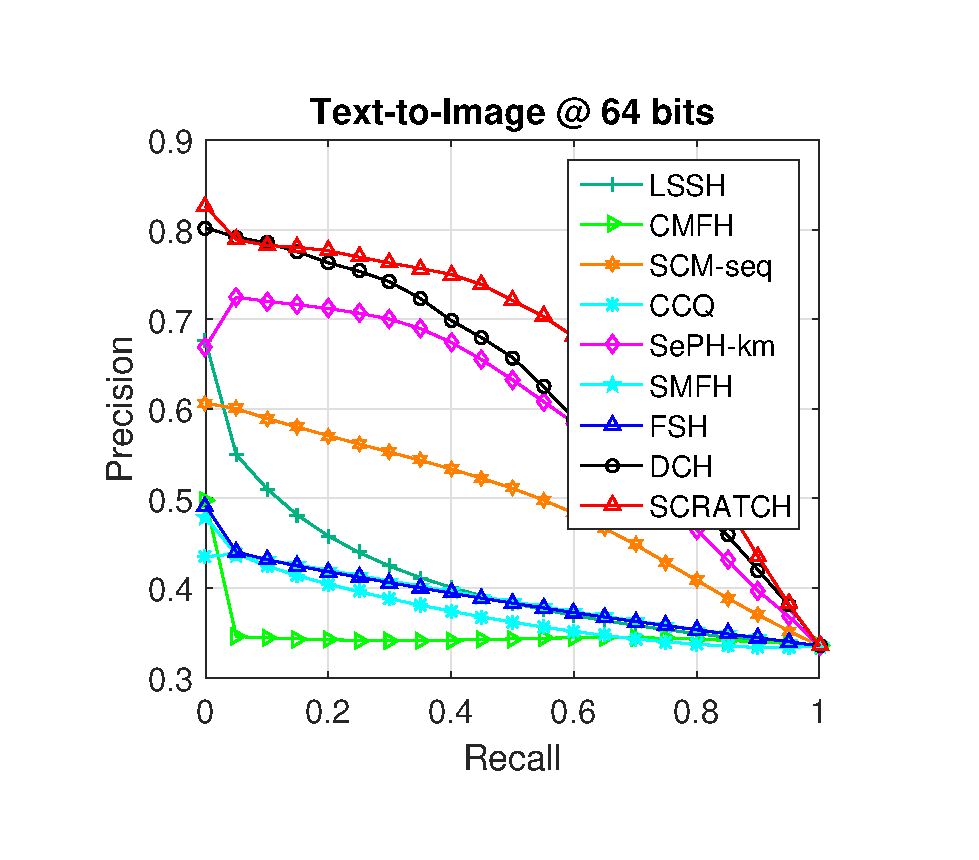
\includegraphics[width=8cm]{figures/NUS_WIDE_P_R/P_R_Text_Vs_Image_64}}
\end{minipage}
%\vspace{-4mm}
\caption{\bf NUS-WIDE ���ݼ�\ 64 λ��ϣ���\ Precision-Recall ����}
\label{curves-nus-3}\medskip
\end{figure*}


\begin{figure*}
\vspace{-12mm}
\begin{minipage}{0.5\linewidth}
\centering
\centerline{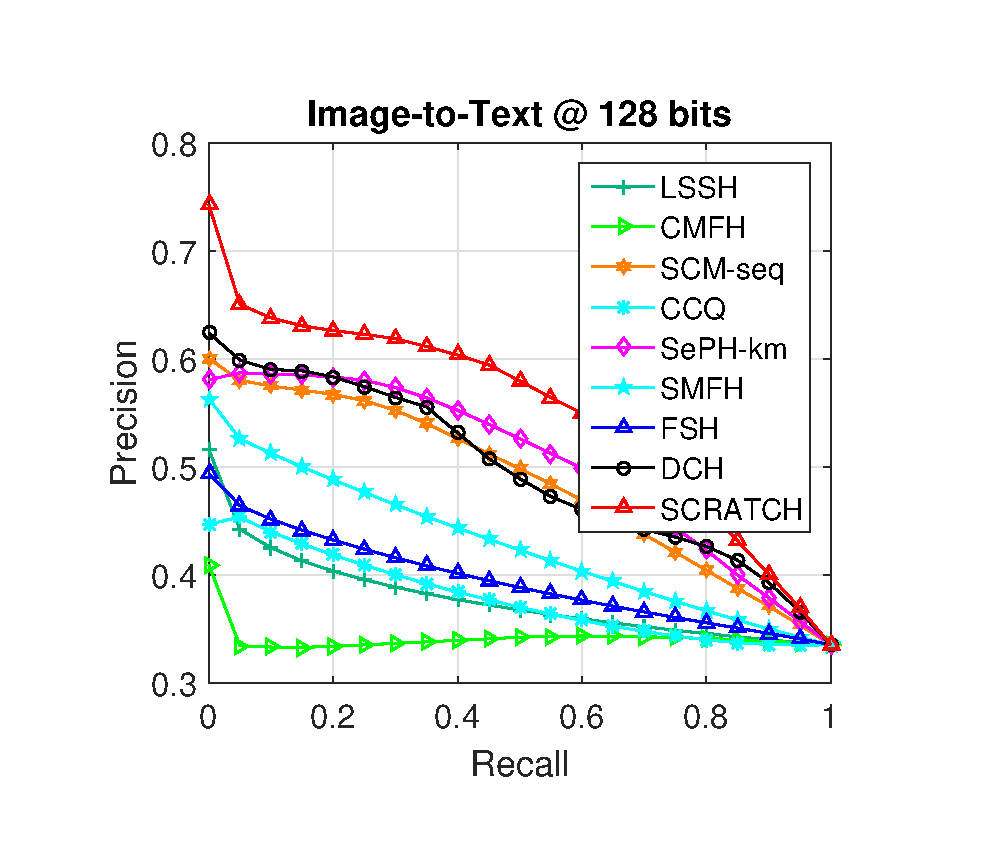
\includegraphics[width=8cm]{figures/NUS_WIDE_P_R/P_R_Image_Vs_Text_128}}
\end{minipage}
%\vspace{-6mm}
\begin{minipage}{0.5\linewidth}
\centering
\centerline{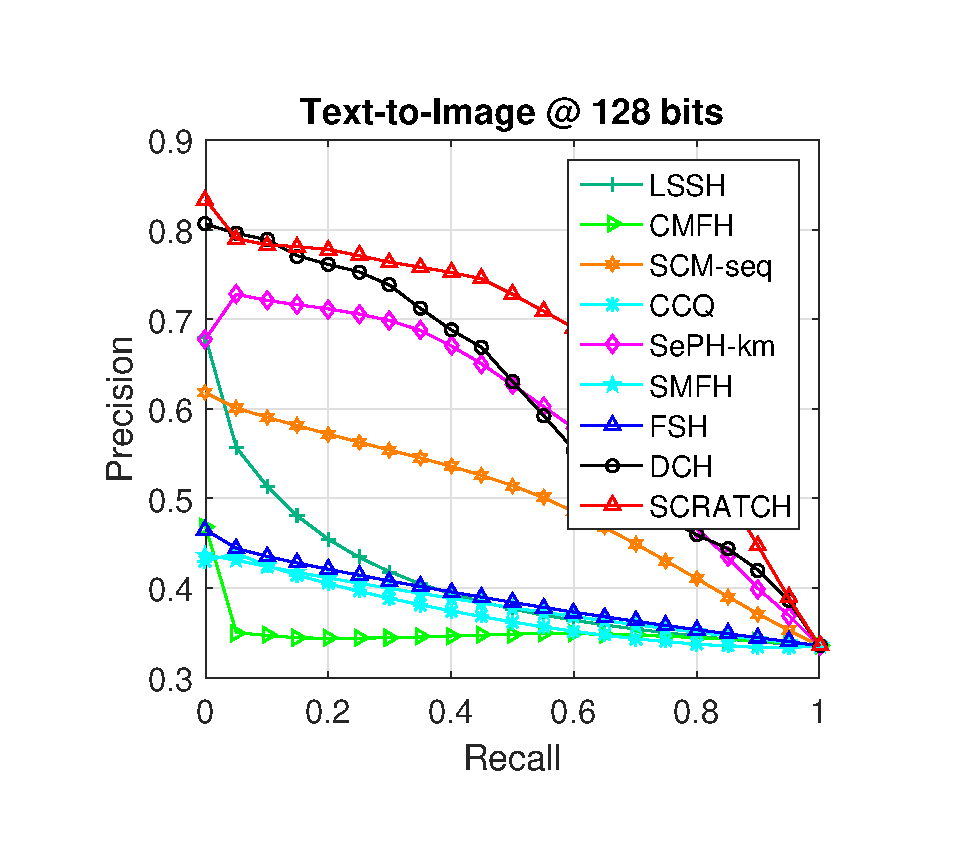
\includegraphics[width=8cm]{figures/NUS_WIDE_P_R/P_R_Text_Vs_Image_128}}
\end{minipage}
\caption{\bf NUS-WIDE ���ݼ�\ 128 λ��ϣ���\ Precision-Recall ����}
\label{curves-nus-4}\medskip
\end{figure*}


\begin{table}[tb]
%\setlength{\belowcaptionskip}{-0.3cm}
\small
\center
\begin{center}
\caption{\bf NUS-WIDE ���ݼ�����\ MAP �����ܶԱ�}
\label{mAP_nus}
%\vspace{-3mm}
\label{NUSWIDEmAP}
\begin{tabular}{cllllll}
  \toprule[1pt]
  Task & Method & 8 bits & 16 bits & 32 bits & 64 bits & 128 bits\\
  \hline
  \multirow{8}{*}{\tabincell{c}{Image\\to\\Text}}
  & {LSSH} & {0.3829} & {0.3885} & {0.3869} & {0.3911} & {0.3877}\\
  & {CMFH} & {0.3406} & {0.3437} & {0.3399} & {0.3409} & {0.3440}\\
  & {SCM-seq} & {0.5013} & {0.5120} & {0.5422} & {0.5488} & {0.5483}\\
  & {CCQ} & {0.3902} & {0.3959} & {0.3929} & {0.4010} & {0.3952}\\
  & {SePH-km} & {0.5256} & {0.5537} &{0.5627} & {0.5622} & {0.5698}\\
  & {SMFH} & {0.3711} & {0.4006} & {0.4461} & {0.4593} & {0.4594}\\
  & {FSH} & {0.3620} & {0.3732} & {0.3894} & {0.4014} & {0.4084}\\
  & {DCH} & {0.5840} & {0.5808} & {0.5907} & {0.5932} & {0.5843}\\
  & {SCRATCH} & {\bf{0.6038}} & {\bf{0.6207}} & {\bf{0.6338}} & {\bf{0.6459}} &{\bf{0.6496}}\\
  \hline
  \multirow{8}{*}{\tabincell{c}{Text\\to\\Image}}
  & {LSSH} & {0.4075} & {0.4202} & {0.3444} & {0.4231} & {0.4175}\\
  & {CMFH} & {0.3456} & {0.3498} & {0.3435} & {0.3486} & {0.3529}\\
  & {SCM-seq} & {0.4709} & {0.4836} & {0.5067} & {0.5141} & {0.5161}\\
  & {CCQ} & {0.3716} & {0.3740} & {0.3712} & {0.3734} & {0.3765}\\
  & {SePH-km} & {0.6102} & {0.6407} & {0.6515} & {0.6608} & {0.6651}\\
  & {SMFH} & {0.3631} & {0.3789} & {0.4046} & {0.4048} & {0.3997}\\
  & {FSH} & {0.3623} & {0.3717} & {0.3835} & {0.3973} & {0.4007}\\
  & {DCH} & {0.7106} & {0.7103} & {0.7098} & {0.7260} & {0.7223}\\
  & {SCRATCH} & {\bf{0.7210}} & {\bf{0.7392}} &{\bf{0.7549}} & {\bf{0.7680}} &{\bf{0.7755}}\\
  \toprule[1pt]
\end{tabular}
\end{center}\smallskip
\end{table}



\subsection{NUS-WIDE ���ݼ�ʵ����}
\esubsection{Results on NUS-WIDE}
\label{sec:nus-wide}

���з�����\ NUS-WIDE ���ݼ��ϵ�\ MAP ʵ�����ڱ�\ \ref{mAP_nus} �н������ܽᣬNUS-WIDE ���ݼ���\ 64 λ��\ 128 λ��ϣ���ϵ�\ top-N precision ��\ precision-recall ������ͼ\ \ref{curves-nus-1}��\ref{curves-nus-4} �л���������Щʵ�����У����ǿ��Եõ����½��ۣ���Щ������\ Wiki ��\ MIRFlickr-25K ���ݼ��ϵ�ʵ��������ƣ�
\begin{itemize}
\vspace{-3mm}
\item SCRATCH �ڸ��������µļ������ܶ�Ҫ���������������жԱȷ�������֤�����ڴ��ģ���ݼ��ϵ�ʵ���ԡ�
\vspace{-3mm}
\item ���Ź�ϣ��λ�����ӣ�SCRATCH �ļ������ܳ���������˵�������Ĺ�ϣ���ܹ���������Ϣ�������ϣ���У��Ӷ�ʵ�ּ������ܵĿ���������
\vspace{-3mm}
\item �����������\ Text-to-Image �����ϵļ�������ҪԶԶ����\ Image-to-Text ���������\ Wiki ��\ MIRFlickr-25K ���ݼ�һ�¡�
\vspace{-3mm}
\item �����мල��ģ̬��ϣ��������\ SCRATCH��DCH��������ҪԶԶ��Խ�������޼ල��������\ CMFH ��\ FSH����˵��������������Ϣ�����ڹ�ϣ��������Ա��֣��Ӷ���������������ܣ���һ��˵�������üල������Ϣ����Ч�ԡ�
\vspace{-3mm}
\item SCRATCH �ڹ�ϣ��λ���ܵͣ���\ 8 ��\ 16 λ����ʱ����Ȼȡ����Զ���������Աȷ����ļ������ܡ�
\vspace{-3mm}
\item SCRATCH ��\ $N$ �dz�С��ʱ��Ҫ�������Աȷ������ָ��ã�������\ Image-to-Text �ϣ�����˵��\ SCRATCH �� \ $N$ ��Сʱ�ܹ������������ѯ��������ص����ݿ���������Լ���������˵�Ƿdz���Ҫ�ġ�
\end{itemize}

�ܶ���֮��SCRATCH ���������û�׼���ݼ���ȡ���˼��߾������ļ������ܣ�˵����ͬʱ�����ʽ�ı�ǩ������Ϣ�ͻ���Эͬ����ֽ��ھ��������������Ϣ���Ը��õؽ������������Եı��֣��Ӷ�ʹ�����ɵĹ�ϣ���������ߡ���������������Эͬ����ֽ�Ŀ�ģ̬��������\ CMFH ��\ SMFH����ȣ�SCRATCH �������������ݼ���ʵ���˸��õļ������ܣ��Ӷ�֤���˱����������ʧ�������Ż�ģʽ����Ч�ԣ��������ڼ����ǩ��������ϢǶ������������ת�������ɢ�Ż���������\ SCRATCH ԶԶ��Խ����������Эͬ����ֽ�Ŀ�ģ̬��ϣ������


\subsection{���������Է���}
\esubsection{Parameter sensitivity analysis}

������ǰ����˵��������׼���ݼ��϶Բ��������Խ������꾡��ʵ�飬ͨ��ÿ�ι̶��������б�����ֻ��һ��������һ����Χ�ڽ��б仯���õ����Ӧ�ı仯���ߣ��Ӷ��ܹ���ֱ�۵ع۲쵽�������������ȡֵ�����У�������\ $\lambda_1$ ��\ $\lambda_2$ ����������ģ̬Эͬ����ֽ����Ȩ�أ��������ǵ�ʵ���з��֣��������������ı仯�����ս����Ӱ��Ƚ�С��������Ǿ����Ե�����������������Ϊ\ $\lambda_1$ = $\lambda_2$ = 0.5������֮�⣬����Ҳ�������������Ե�ʵ����˵�����������\ SCRATCH �����ں��ٵ�ѵ������������ﵽ����״̬���Ӷ�ʵ�ֿ��ٵ�ѵ���Ż������Գ�����\ $\mu$��$\alpha$��$\gamma$ ���б仯ʱ����Ӧ���������ݼ���\ 64 λ��ϣ�����������ģ̬����������ȡ�õ� MAP ������ͼ\ \ref{curves-param-1} ��\ \ref{curves-param-2} �и�����ͬʱ�������ݼ���Ŀ�꺯��ֵ���ڵ��������ı仯Ҳ��ͼ\ \ref{curves-param-2} �л���������\ ``I-T'' ��\ ``T-I'' �ֱ����\ Image-to-Text ��\ Text-to-Image ���񡣴�����ʵ���������ǿ��Եó����¹۲�ͽ��ۣ�


\begin{figure}
\setlength{\belowcaptionskip}{-0.5cm}
%\vspace{-6mm}
\begin{minipage}{0.5\linewidth}
\centering
\centerline{\includegraphics[width=8cm]{figures/Parameters/lambda}}
\end{minipage}
%\vspace{-6mm}
\begin{minipage}{0.5\linewidth}
\centering
\centerline{\includegraphics[width=8cm]{figures/Parameters/alpha}}
\end{minipage}
\caption{\bf ���ڳ�����\ $\mu$ ��\ $\alpha$ �IJ��������Է���}
\label{curves-param-1}
\end{figure}

\begin{figure}
\setlength{\belowcaptionskip}{-0.5cm}
\vspace{6mm}
\begin{minipage}{0.5\linewidth}
\centering
\centerline{\includegraphics[width=8cm]{figures/Parameters/gamma}}
\end{minipage}
%\vspace{-6mm}
\begin{minipage}{0.5\linewidth}
\centering
\centerline{\includegraphics[width=8cm]{figures/Parameters/convergence}}
\end{minipage}
%\vspace{-3mm}
\caption{\bf ���ڳ�����\ $\gamma$ �͵��������IJ��������Է���}
\label{curves-param-2}
\end{figure}

\begin{itemize}
\vspace{-3mm}
\item \ $\mu$ ��\ $\alpha$ ȷʵ��Ӱ��\ SCRATCH �����ܣ�SCRATCH ��\ $\mu\approx1,000$ ��\ $\alpha\approx500$ ʱȡ�����Ž����
\vspace{-3mm}
\item ��\ $\mu$ ��\ $\alpha$ ��������ʱ��SCRATCH �����ܻ������½�������ζ�ŷ�����ӳ��ͱ�ǩ������Ƕ���ڱ��ķ���������������Ҫ�����á�
\vspace{-3mm}
\item \ $\gamma$ �������������Ȩ�أ���\ $\gamma\approx5$ ʱ\ SCRATCH ȡ�õļ�����������õġ�ֵ��һ����ǣ���\ $\gamma$ ������ʱ��SCRATCH ��\ Wiki ���ݼ��ϵļ������ܼ����½���Ȼ����\ MIRFlickr-25K ��\ NUS-WIDE ������Խϴ��ģ�����ݼ�����û�����������֣����ܵ�ԭ��Ϊ\ Wiki ���ݼ���һ��С���ݼ�������������С�ᵼ��\ SCRATCH �dz����׹���ϣ������������������������˷dz���Ҫ�ı������ϵ����ã�Ȼ��\ MIRFlickr-25K ��\ NUS-WIDE �������ݼ������ݹ�ģ����㹻�����\ SCRATCH �����������ݼ��ϲ����׷�����������󣬴Ӷ���������������ò������ԡ�
\vspace{-3mm}
\item SCRATCH �������������ݼ��Ͼ����ں��ٵĵ����������������״̬����һ��֤ʵ�˱���������Ż����Ե���Ч�Ժ�ʵ���ԡ�
\end{itemize}




\subsection{ʱ�����ķ���}
\esubsection{Time cost analysis}

Ϊ����֤���������\ SCRATCH ģ�͵���Ч�ԣ����ǽ�һ����\ MIRFlickr-25K ���ݼ��ϱȽ������з�����ѵ��ʱ�䣨����Ϊ��λ��ʱ������ϣ�볤��ȡ\ 8��16��32��64 ��\ 128 λ���Ӷ�����ֱ�۵ؿ�����ϣ��λ����ѵ��ʱ���Ӱ�죬���յ�ʵ�����ڱ�\ \ref{training_time} �н���չʾ����ʵ�������Կ��������Ź�ϣ��λ�������ӣ�SCRATCH ��ѵ��ʱ�䲢û���������ӣ�˵��\ SCRATCH ���Է���ĶԸ�ά���ݽ��п�ģ̬��ϣѧϰ������\ CMFH ���޼ල��ģ̬��ϣ������������жԱȷ�����ֻ��\ CMFH ��ѵ���ٶȿ���\ SCRATCH��Ȼ��������ǰ��С�������ģ����ǵ��ٶȺͼ������ȵ�ƽ�⣬CMFH�ļ�������ҪԶԶ����\ SCRATCH�������ۺ϶෽�濼�Ǽ����ٶȺͼ������ȵȣ�SCRATCH ���������ݼ��Ͼ��������ã�����\ SCRATCH ����Ч�ҷ������չ�����ģ���ݼ��ϡ�

\begin{table}[t]
\centering
\small
\caption{\bf MIRFlickr-25K ���ݼ��ϵ�ѵ��ʱ��Աȣ������ʱ��}
\label{training_time}
\resizebox{12cm}{!}{
\begin{tabular}{lrrrrrr}
\toprule[1pt]
%\hline
\multirow{1}{*}{Method}    & 8 bits & 16 bits & 32 bits & 64 bits & 128 bits \\
\hline
 {LSSH}  & {34.41} & {29.89} & {29.67} & {32.44} & {38.17} \\
 {CMFH} & {1.48} & {1.58} & {1.57} & {1.64} & {1.90}\\
 {SCM-seq} & {8.84} & {12.65} & {22.90} & {42.85} & {77.33}\\
 {CCQ} & {6.33} & {9.12} & {17.26} & {29.33} & {77.41}\\
 {SePH-km} & {3328.20} & {3411.26} & {3576.82} & {3805.26} & {4451.09}\\
 {SMFH} & {7.32} & {6.89} & {15.40} & {14.60} & {16.84}\\
 {FSH} & {109.59} & {108.25} & {107.52} & {109.73} & {115.55}\\
 {DCH} & {3.76} & {4.36} & {5.49} & {11.56} & {37.36}\\
 {SCRATCH} & {1.59} & {1.59} & {1.88} & {2.44} & {3.68}\\
\toprule[1pt]
\end{tabular}
}
\setlength{\belowcaptionskip}{-0.5cm}
\smallskip
\end{table}



\begin{table}[b]
\setlength{\abovecaptionskip}{-0.5cm}
\small
\center
\setlength{\abovecaptionskip}{0.1cm}
\begin{center}
\caption{\bf MIRFlickr-25K ���ݼ���\ SCRATCH ��\ DCMH ��\ MAP\ �Ա�}
\label{deep_extension}
\begin{tabular}{cllllll}
  \toprule[1pt]
  Task & Method & 8 bits & 16 bits & 32 bits & 64 bits & 128 bits\\
  \hline
  \multirow{2}{*}{\tabincell{c}{$I\rightarrow T$}}
  & {DCMH} & {0.7276} & {0.7247} & {0.7435} & {0.7484} & {0.7571}\\
  & {SCRATCH} & {\bf{0.7587}} & {\bf{0.7803}} &{\bf{0.7978}} & {\bf{0.8093}} &{\bf{0.8230}}\\
  \hline
  \multirow{2}{*}{\tabincell{c}{$T\rightarrow I$}}
  & {DCMH} & {0.7453} & {0.7580} & {0.7692} & {0.7758} & {0.7819}\\
  & {SCRATCH} & {\bf{0.7532}} & {\bf{0.7797}} &{\bf{0.7913}} & {\bf{0.7979}} & {\bf{0.8160}}\\
  \toprule[1pt]
\end{tabular}
\end{center}
\smallskip
\end{table}


\subsection{����ȹ�ϣ�����Ա�}
\esubsection{Comparison with Deep Hashing}

Ϊ��˵�������������ʧ�������Ż���������Ч�ԣ����ǽ�һ����\ MIRFlickr-25K ���ݼ�����һ����ǰ���ܽϺõ���ȿ�ģ̬��ϣ��DCMH��\cite{jiang2017dcmh}������ʵ��Աȡ���ѭ\ DCMH ��ʵ�����ã��������Ƚ�����\ DCMH ��ʹ�õ�\ CNN-F\cite{ken14cnnf} ������ȡ��ͼ��ģ̬�����������Ȼ���ڵõ������ͼ��������ԭʼ���ı�������ʹ��\ SCRATCH ���п�ģ̬��ϣ���������յ�\ MAP ʵ�����ڱ�\ \ref{deep_extension} �н������ܽᣬ�ӽ���п��Եó����¹۲죺
\begin{itemize}
\vspace{-3mm}
\item SCRATCH ��������ģ̬���������ϵ����ܾ�������\ DCMH��
\vspace{-3mm}
\item ���Ź�ϣ��λ�����ӣ�SCRATCH �ļ������ܳ���������˵�������Ĺ�ϣ���ܹ���������Ϣ�������ϣ���У��Ӷ�ʵ�ּ������ܵĿ���������
\vspace{-3mm}
\item SCRATCH ��\ Image-to-Text �����ϵ����Ź�ϣ��λ���ı仯���������ܾ��������\ DCMH��
\vspace{-3mm}
\item SCRATCH ����������ϵ�\ Image-to-Text ��������ҪԶԶ�������˹���ȡ�����ϵ����ܣ���ʹ�����ͼ��������\ SCRATCH �ڹ�ϣ��λ���ܵͣ���\ 8 ��\ 16 λ��ʱ\ Image-to-Text ����ļ��������Ѿ�������ʹ���˹�����\ SCRATCH �ڸ�λ��ϣ�루128 λ�������ܣ�˵����Ⱦ�����������ȡ����ͼ����������Խ�ԡ�
\end{itemize}



%
%\subsection{������չ}
%\esubsection{Extension to classification}
%
%
%
%\begin{table*}[t]\scriptsize
%\caption{CLASSIFICATION performance comparison of various models on MIRFlickr-25000 and NUS-WIDE.}\label{table_classification}
%\centering
%\begin{tabular}{cccccccccccccc}
%\toprule[1pt]
%\multirow{3}{*}{Task} & \multirow{3}{*}{Method} & \multicolumn{6}{c}{MIRFlickr} & \multicolumn{6}{c}{NUS-WIDE}\\
%\cmidrule(lr){3-8} \cmidrule(lr){9-14}
%&& \multicolumn{3}{c}{MacroF1} & \multicolumn{3}{c}{Accuracy} & \multicolumn{3}{c}{MacroF1} & \multicolumn{3}{c}{Accuracy} \\
%
%\cmidrule(lr){3-5}  \cmidrule(lr){6-8} \cmidrule(lr){9-11} \cmidrule(lr){12-14} & &16 bits & 32 bits & 64 bits & 16 bits & 32 bits & 64bits & 16 bits & 32 bits & 64 bits & 16 bits & 32 bits & 64bits\\ \hline
%\multirow{8}{*}{\tabincell{c}{ Image }}
%
% {}&CVH & 0.0627 & 0.0486 & 0.0463 & 0.1428 & 0.1229 & 0.1184  & 0.1129 & 0.0858 & 0.0651 & 0.1648 & 0.1394 & 0.1288 \\
% {}&IMH & 0.0521 & 0.0586  &0.0590& 0.0998& 0.1207 & 0.1250 & 0.0806 & 0.0890  &0.1001& 0.1021& 0.1060 & 0.1233 \\
% {}&SCM-seq  & 0.0834 & 0.0820& 0.0900 & 0.1580 & 0.1642& 0.1814 & 0.2062 & 0.1985& 0.2159& 0.3051 & 0.2798& 0.3066\\
% {}&LSSH & 0.0750 & 0.0722 & 0.1115 & 0.1144 & 0.1106 & 0.1653 & 0.1908 & 0.2030 & 0.2227 & 0.2283 & 0.2362 & 0.2781 \\
% {}&CMFH & 0.0824 & 0.0243 & 0.0265 & 0.1488 & 0.0831 & 0.0830 & 0.0505 & 0.0492 & 0.0484 & 0.1075 & 0.1098 & 0.1093 \\
% {}&FSH & 0.0801 & 0.0874 & 0.0910 & 0.1415 & 0.1410 & 0.1448 & 0.1623 & 0.2026 & 0.2320 & 0.2324 & 0.2915 & 0.3132 \\
% {}&SePH-km & 0.1664 & 0.1926 & 0.1997 & 0.2719 & 0.2704 & 0.2732 & 0.2718 & 0.2781 & 0.2561 & 0.3520 & 0.3470 & 0.3414\\
% {}&SRDMH & \textbf {0.2240} & {\textbf{0.2554}} & {\textbf{0.2784}} & {\textbf{0.2793}} & {\textbf{0.2710}} & {\textbf{0.2749}} & \textbf {0.2919} & {\textbf{0.3036}} & {\textbf{0.4251}}& {\textbf{0.3702}} & {\textbf{0.3896}} & {\textbf{0.4207}} \\
%\hline
%\multirow{8}{*}{\tabincell{c}{ Text }}
% {}&CVH & 0.0716 & 0.0673 & 0.0758 &0.1565 & 0.1482 & 0.1513 & 0.1497 & 0.1580 & 0.1652 &0.2222 & 0.2170 & 0.2296 \\
% {}&IMH & 0.0458 & 0.0688 & 0.1218 &0.0893 & 0.1156 & 0.1637 & 0.0732& 0.1424 & 0.2158 &0.0815& 0.1581 & 0.2477 \\
% {}&SCM-seq & 0.1682 & 0.2464 & 0.3125 & 0.3187 & 0.3597 & 0.3830 & 0.3770& 0.4336 & 0.4765 & {\textbf {0.4933}} & 0.5028 & 0.5357\\
% {}&LSSH & 0.1343 & 0.2033 & 0.2503  & 0.1495 & 0.1966 & 0.2622 & 0.2794& 0.3060 & 0.3422  & 0.3326 & 0.3492 & 0.3958\\
% {}&CMFH & 0.1068 & 0.0312 & 0.0314& 0.1838 & 0.0806 & 0.0806 & 0.0519 & 0.0504 & 0.0502 & 0.1114 & 0.1115 & 0.1087\\
% {}&FSH & 0.0738 & 0.0882 & 0.0992  & 0.1270 & 0.1454 & 0.1637 & 0.1650& 0.2294 & 0.2747 & 0.2242 & 0.3269 & 0.3677\\
% {}&SePH-km & 0.2135 & 0.2802 & 0.2818& 0.3353 & 0.3807 & 0.3860 & 0.4021 & 0.4225 & 0.3957 & 0.4923 & 0.5026 & 0.5048 \\
% {}&SRDMH & {\textbf {0.3018}} & {\textbf{0.3658}} & {\textbf{0.4085}}& {\textbf {0.3375}} & {\textbf{0.3824}} & {\textbf{0.3867}} & \textbf {0.4022} & {\textbf{0.4545}} & {\textbf{0.5608}}& {\textbf{0.4933}} & {\textbf{0.5069}} & {\textbf{0.5387}} \\\hline
%\toprule[1pt]
%\end{tabular}
%\end{table*}

\section{������}
\esection{Summary}

��������ͨ��\ MAP �Աȡ�top-N precision ��\ precision-recall �����Լ�ѵ��ʱ��Աȵ�ʵ�����������֤��\ SCRATCH ����Ч�ԣ�ͬʱ����ȿ�ģ̬��ϣ�����Աȣ�����ʹ����Ⱦ����������\ SCRATCH ����һ���˵��˵����ģ�ͣ�����ͬʱѵ�������\ SCRATCH ģ�ͣ�������ȡ��ģ��ѵ���Ƿֿ��ģ���������Ȼȡ���˳�Խ��ǰ�Ƚ�����ȿ�ģ̬��ϣ������DCMH���ļ������ܣ����һ��˵����\ SCRATCH ���õ���ʧ�������Ż����Ե��Ƚ��Ժ���Ч�ԡ�


\input{./Chapters/conclusions}
%\input{./Chapters/chap4}
%\input{./Chapters/chap5}
%\input{./Chapters/chap6}
\SDUbackmatter

\ereference{Reference}
\bibliographystyle{SDUthesis}
%\bibliographystyle{unsrt}
\bibliography{thesisbib}

\begin{thanks}
\ethanks{Acknowledgements}

ʱ����ţ�������о������ļ���������Ҳ�����ż��������������������԰��ɽ�¸�𣬸п���ǧ��

��л�ҵ��о�����ʦ����˳��ʦ���ӱ��ƴ����Ŀ������ֿ�ʼ�ͽ���������ʦ�Ľ̵����������������ʦԨ����ѧʶ���������ɼ��Ŀ���̬�ȣ�
֮�����̸��ֹ�����˽��������д������Ŀ�滮���������޾�ϸ��������Ϊ������˵����ʦҲ���ҽ��̤������������ʦ���ڹ���ʵϰ�ȷ���
����ʦҲ����΢������������������ʦ��Ϊ�ҵ���·�ˣ��ڴ�������ʦ���������ֿ�ĸ�л��

��лʵ���ҵ�С����ǣ��о�������ʱ�䣬�Ҵ�ѧ�ܰ�����ѧ�����Ӹ���ʱ���ͷ�ൽ������ʦ�֣���л��ҵİ��ݺ����£�Ҳ��л����Ӫ���˻�����Ǣ��ʵ���ҷ�Χ�������ܹ��������ضȹ��о������ġ�

��л����ӵ��ֵ��ǣ��������������ҵ����ң��ܸ�����������һ��ƴ������һֱ���ֻ�������̬��ϣ���л��ỹ��һ�����������Ϣ������ֹ��

��л�ҵļ��˺ͻ�������л�������Ҿ�ɥ�Ľ׶θ����ҹ��ĺ͹�����û�����ǵ�������޷����˳�������ѧҵ��Ը��������˳�ģ��Ҹ�������

��󣬸�л���а�����֧���ҵ��ˣ���ҵ���ǽ������µ�����ոտ�ʼ���Ҷ����Ļ��ж����������ģ�����ǰ�У�


\end{thanks}
%\cleardoublepage

%\cleardoublepage


\input{./Chapters/publications}

\end{document}
